\documentclass[12pt]{book}
\usepackage{fontspec}
\setmainfont{TeX Gyre Pagella}
\usepackage[paperwidth=8in,paperheight=8in,margin=0.6in]{geometry}
\usepackage{xcolor}
\usepackage{amssymb}
\usepackage{tikz}
\usetikzlibrary{arrows.meta}
\pagestyle{empty}
\setlength{\parindent}{0pt}

\newcommand{\artnote}[1]{{\color{gray!70}\small\itshape [Illustration: #1]}\par\vspace{0.3in}}
\newcommand{\bigline}[1]{{\Huge #1}\par}
\newcommand{\pagenum}[1]{\vfill{\color{gray!50}\footnotesize #1}}
\newcommand{\sprollpage}{\newpage\vspace*{0.4in}}
\newcommand{\groupscene}{%
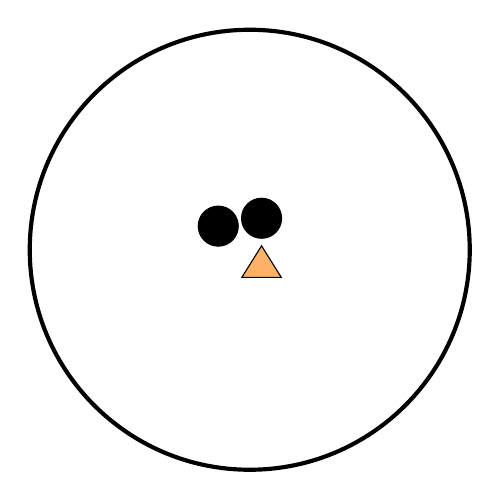
\begin{tikzpicture}
\draw[line width=1.5pt] (0,0) circle (1.1in);
\filldraw[fill=black] (-0.4,0.3) circle (0.1in);
\filldraw[fill=black] (0.15,0.4) circle (0.1in);
\draw[fill=orange!60] (-0.1,-0.35) -- (0.15,0.05) -- (0.4,-0.35) -- cycle;
\end{tikzpicture}}

\begin{document}

\thispagestyle{empty}
\begin{center}
\vspace*{1.1in}
{\Huge \textbf{SPROLL 06}}\\[0.4in]
{\huge \textbf{Look Through a Rule}}\\[0.5in]
\groupscene
\\[0.3in]
{\large \textit{the same group, seen different ways}}\\[0.3in]
{\small The Sproll Curriculum $\cdot$ Cycle I: Pops}
\end{center}

\sprollpage
\begin{center}
\vspace*{1.5in}
{\Large The Sproll Curriculum}\\[0.2in]
{\normalsize Cycle I --- Pops: Things, Differences, and Counting}\\[0.6in]
{\small Sproll 06 of 40 \quad $\cdot$ \quad follows Sproll 05: Together}
\end{center}
\pagenum{2}

\sprollpage
\begin{center}
\vspace*{0.5in}
\artnote{a boundary containing two dots and a triangle, the familiar group scene}
\groupscene
\vspace{0.3in}
\bigline{How many things are here?}
\end{center}
\pagenum{3}

\sprollpage
\begin{center}
\vspace*{0.9in}
\artnote{the same group, small and unchanged, off to one side, with empty space for the answer}
\groupscene
\vspace{0.35in}
\bigline{It depends on how you look.}
\end{center}
\pagenum{4}

\sprollpage
\begin{center}
\vspace*{0.5in}
\artnote{the same group, with a label above it reading a rule, and a large numeral 3 beneath it}
\groupscene
\vspace{0.15in}
{\large Rule: count everything.}
\vspace{0.15in}\\
{\Huge \textbf{3}}
\end{center}
\pagenum{5}

\sprollpage
\begin{center}
\vspace*{0.5in}
\artnote{the same group, with the two dots highlighted and the triangle faded, and a numeral 2 beneath}
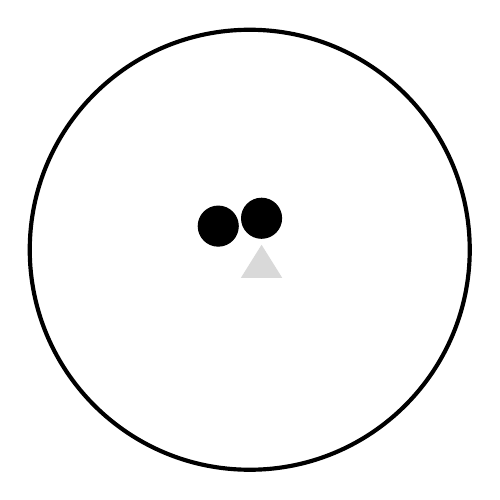
\begin{tikzpicture}
\draw[line width=1.5pt] (0,0) circle (1.1in);
\filldraw[fill=black] (-0.4,0.3) circle (0.1in);
\filldraw[fill=black] (0.15,0.4) circle (0.1in);
\draw[fill=orange!60, gray!30, draw=gray!30] (-0.1,-0.35) -- (0.15,0.05) -- (0.4,-0.35) -- cycle;
\end{tikzpicture}
\vspace{0.15in}
{\large Rule: count only the round ones.}
\vspace{0.15in}\\
{\Huge \textbf{2}}
\end{center}
\pagenum{6}

\sprollpage
\begin{center}
\vspace*{0.5in}
\artnote{the same group, with the triangle highlighted and the two dots faded, and a numeral 1 beneath}
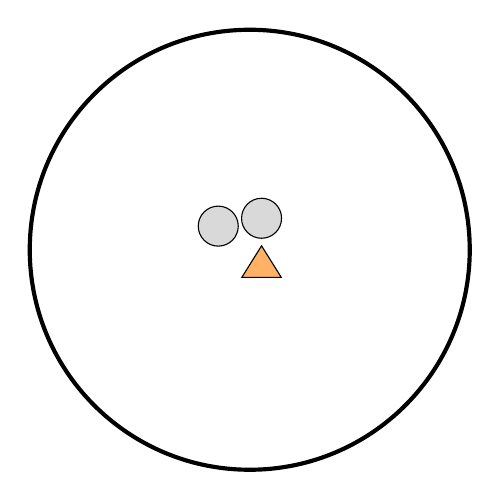
\begin{tikzpicture}
\draw[line width=1.5pt] (0,0) circle (1.1in);
\filldraw[fill=gray!30] (-0.4,0.3) circle (0.1in);
\filldraw[fill=gray!30] (0.15,0.4) circle (0.1in);
\draw[fill=orange!60] (-0.1,-0.35) -- (0.15,0.05) -- (0.4,-0.35) -- cycle;
\end{tikzpicture}
\vspace{0.15in}
{\large Rule: count only the pointy ones.}
\vspace{0.15in}\\
{\Huge \textbf{1}}
\end{center}
\pagenum{7}

\sprollpage
\begin{center}
\vspace*{0.5in}
\artnote{the three previous answers, 3, 2, and 1, shown together in a row, all beneath the same unchanged group}
\groupscene
\vspace{0.15in}
{\Large 3 \quad\quad 2 \quad\quad 1}
\vspace{0.25in}
\bigline{Same group.}\vspace{0.1in}
{\Large Different rules.}\\
{\Large Different answers.}\\
{\Large All correct.}
\end{center}
\pagenum{8}

\sprollpage
\begin{center}
\vspace*{0.7in}
\artnote{the group scene once more, now with a small labeled lens or magnifying frame held up in front of it}
\groupscene
\vspace{0.3in}
\bigline{Looking at something through a rule,}\vspace{0.1in}
{\Large to get one answer, is called a Collapse.}
\end{center}
\pagenum{9}

\sprollpage
\begin{center}
\vspace*{0.5in}
\artnote{the same group shown twice: once with the shapes scattered in their original positions, once redrawn in a tidy row, same three shapes, positions ignored}
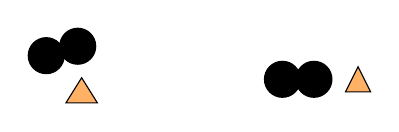
\begin{tikzpicture}
\filldraw[fill=black] (-2.3,0.3) circle (0.09in);
\filldraw[fill=black] (-1.9,0.42) circle (0.09in);
\draw[fill=orange!60] (-2.05,-0.3) -- (-1.85,0.02) -- (-1.65,-0.3) -- cycle;
\filldraw[fill=black] (0.7,0) circle (0.09in);
\filldraw[fill=black] (1.1,0) circle (0.09in);
\draw[fill=orange!60] (1.5,-0.16) -- (1.66,0.16) -- (1.82,-0.16) -- cycle;
\end{tikzpicture}
\vspace{0.3in}
\bigline{Rule: ignore where things are.}\vspace{0.1in}
{\Large Same three shapes, tidied up.}
\end{center}
\pagenum{10}

\sprollpage
\begin{center}
\vspace*{0.5in}
\artnote{the mixed ledger from Sproll 05 (a Pop, another Pop, a Bind entry), with a rule label above it and a numeral 3 beneath}
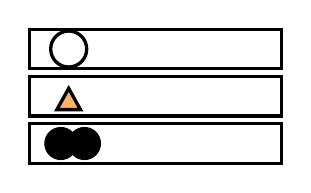
\begin{tikzpicture}
\draw[line width=1.2pt] (-1.6,0.7) rectangle (1.6,1.2);
\draw[line width=1.2pt] (-1.1,0.95) circle (0.09in);
\draw[line width=1.2pt] (-1.6,0.1) rectangle (1.6,0.6);
\draw[fill=orange!60, line width=1.2pt] (-1.25,0.18) -- (-1.1,0.45) -- (-0.95,0.18) -- cycle;
\draw[line width=1.2pt] (-1.6,-0.5) rectangle (1.6,0);
\filldraw[fill=black] (-1.2,-0.25) circle (0.08in);
\filldraw[fill=black] (-0.9,-0.25) circle (0.08in);
\draw[line width=1.2pt] (-1.08,-0.25) -- (-1.02,-0.25);
\end{tikzpicture}
\vspace{0.2in}
{\large Rule: count every entry.}\\
{\Huge \textbf{3}}
\end{center}
\pagenum{11}

\sprollpage
\begin{center}
\vspace*{0.5in}
\artnote{the same ledger, with only the first two lines highlighted and the Bind line faded, numeral 2 beneath}
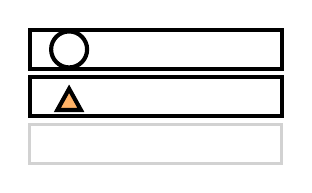
\begin{tikzpicture}
\draw[line width=1.5pt] (-1.6,0.7) rectangle (1.6,1.2);
\draw[line width=1.5pt] (-1.1,0.95) circle (0.09in);
\draw[line width=1.5pt] (-1.6,0.1) rectangle (1.6,0.6);
\draw[fill=orange!60, line width=1.5pt] (-1.25,0.18) -- (-1.1,0.45) -- (-0.95,0.18) -- cycle;
\draw[line width=1pt, gray!35] (-1.6,-0.5) rectangle (1.6,0);
\end{tikzpicture}
\vspace{0.2in}
{\large Rule: count only the Pops.}\\
{\Huge \textbf{2}}
\end{center}
\pagenum{12}

\sprollpage
\begin{center}
\vspace*{0.8in}
\artnote{a blank ledger with a question mark where a rule label should be}
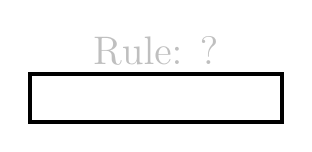
\begin{tikzpicture}
\draw[line width=1.5pt] (-1.6,-0.3) rectangle (1.6,0.3);
\node[gray!50] at (0,0.6) {\Large Rule: ?};
\end{tikzpicture}
\vspace{0.35in}
\bigline{Without a rule,}\vspace{0.1in}
{\Large ``how many'' has no single answer.}
\end{center}
\pagenum{13}

\sprollpage
\begin{center}
\vspace*{0.6in}
\artnote{a brand new small group -- one dot, one triangle, one square -- ready for the reader to try a Collapse of their own}

\begin{tikzpicture}
\filldraw[fill=black] (-1.1,0) circle (0.14in);
\draw[fill=orange!60] (-0.15,-0.2) -- (0.1,0.22) -- (0.35,-0.2) -- cycle;
\draw[line width=2pt] (0.9,-0.2) rectangle (1.4,0.2);
\end{tikzpicture}
\vspace{0.35in}
\bigline{Choose your own rule.}\vspace{0.1in}
{\Large How many things does it count?}
\end{center}
\pagenum{14}

\sprollpage
\begin{center}
\vspace*{0.6in}
\artnote{the original two-dots-and-triangle group once more, calm and unchanged}
\groupscene
\vspace{0.3in}
\bigline{What you see depends}\vspace{0.1in}
{\Large on which rule you choose to look through.}
\vspace{0.35in}\\
{\small \textit{--- turn the page for Sproll 07: Same Picture, Different Story ---}}
\end{center}
\pagenum{15}

\sprollpage
\vspace*{0.3in}
{\large \textbf{A Note for Grown-Ups}}
\vspace{0.2in}

\normalsize
This book introduces Collapse: observing a constructed history or group through a chosen rule to produce one definite answer, with different rules legitimately producing different, equally correct answers from the exact same underlying thing. This is also the first book in the series in which anything is calculated; every earlier book built, chose, refused, or connected, but never evaluated.

\vspace{0.15in}
The examples deliberately span two kinds of ``thing being observed'': a static group of shapes, and a growing record (the ledger introduced in Sproll 02 and extended in Sprolls 04 and 05). The same Collapse idea applies to both. A rule that says ``count everything'' or ``count only the Pops'' is doing exactly the same kind of work as a rule that says ``count only the round ones.''

\vspace{0.15in}
Ordinary arithmetic evaluation, which children typically meet as an unquestioned given, is being quietly introduced here as one particular Collapse rule among many possible ones, not as a special operation with its own separate status. This groundwork matters for later books in the series that revisit exactly what a picture, or a calculation, keeps and discards.

\vspace{0.3in}
{\small Sproll 07: Same Picture, Different Story continues directly from this book's final page.}
\pagenum{16}

\end{document}
